\documentclass{article}
%include polycode.fmt
%
% %s/{lattice-\(.*\)}/{..\/images\/lattice-\1.png}/
% %s/{cat-\(.*\)}/{..\/images\/cat-\1.png}/
%
\begin{document}
This post contains excerpts from \href{https://oleg.fi/pdfs/Monotone.pdf}{a PDF "post" I have written}.
It looks way better in PDF.

\emph{Partial ordered set}, or poset for short is well used example in
category theory books.
Yet, posets are not too familiar for an average
CT-curious Haskeller, yet they are easy to visualise!
Let's do exactly that, and mention elementery bits of category theory.
In particular, I'll scan over the six first chapters of
\emph{Category Theory} by Steve Awodey,
repeating related definitions and poset examples.\footnote{%
If you want to learn category theory, getting a book is a small investment.
Your public or university library probably have a copy.
}

\section{Categories}
\label{sec:categories}

\begin{definition}[Awodey 1.1]\textbf{Definition} (Awodey 1.1)
A \emph{category} consist of the following data
\begin{itemize}
\item Objects: $A, B, C, \ldots$
\item Arrows: $f, g, h, \ldots$

\item For each arrow $f$, there are given objects

\begin{equation*}
\mathrm{dom}(f), \qquad \mathrm{cod}(f)
\end{equation*}

called the \emph{domain} and \emph{codomain} of $f$. We write

\begin{equation*}
f : A \to B
\end{equation*}

to indicate that $A = \mathrm{dom}(f)$ and $B = \mathrm{cod}(f)$.

\item Given arrows $f : A \to B$ and $g : B \to C$, that is, with

\begin{equation*}
\mathrm{cod}(f) = \mathrm{dom}(g)
\end{equation*}

there is given an arrow

\begin{equation*}
g \circ f : A \to C
\end{equation*}

called the \emph{composite} of $f$ and $g$.

\item For each object $A$, there is given an arrow

\begin{equation*}
1_A : A \to A
\end{equation*}

called the \emph{identity arrow} of $A$.

\item Associativity:

\begin{equation*}
h \circ (g \circ f) = (h \circ g) \circ f
\end{equation*}

for all $f : A \to B$, $g : B \to C$, $h : C \to D$.

\item Unit:

\begin{equation*}
f \circ 1_A = f = 1_B \circ f
\end{equation*}

for all $f : A \to B$.
\end{itemize}
\end{definition}

We'll see how |Category| type-class is related later, in later section.

\rule{\textwidth}{1pt}
\ldots
\rule{\textwidth}{1pt}

\section{Functor}

Before proceeding, we'll answer a question: is there a category
with posets as objects? Yes, it's called $\mathbf{Pos}$!
What are the arrows in this category?
An arrow from a poset $A$ to a poset $B$ is a function

\begin{equation*}
m : A \to B
\end{equation*}

that is \emph{monotone}, in the sense that, for all $a, a' \in A$,

\begin{equation*}
a \le_A a' \qquad\text{implies}\qquad m(a) \le_B m(a').
\end{equation*}

We need to know that $1_A : A \to A$ is monotone, and also
that if $f : A \to B$ and $g : B \to C$ are monotone, then $g \circ f : A \to C$
is monotone. That holds, check!

Recall, posets are categories, so monotone functions are "mappings" between
categories. A "homomorphism\footnote{morphism preserving the structure} of categories"
is called a functor.

\begin{definition}[Awodey 1.2]\textbf{Definition} (Awodey 1.2)
A \emph{functor}

\begin{equation*}
F : \mathbf{C} \to \mathbf{D}
\end{equation*}

between categories $\mathbf{C}$ and $\mathbf{D}$ is a mapping of objects
to objects and arrows to arrows, in such a way that
\begin{itemize}
\item $F (f : A \to B) = F(f) : F(A) \to F(B)$,
\item $F(1_A) = 1_{F(A)}$,
\item $F(g \circ f) = F(g) \circ F(f)$.
\end{itemize}
That is, $F$ preserves domains and codomains, identity arrows,
and composition. A functor $F : \mathbf{C} \to \mathbf{D}$ thus gives
a sort of "picture" -- perhaps distorted -- of $\mathbf{C}$ in $\mathbf{D}$.
\end{definition}

The \Haskell\ version looks quite different:
\begin{code}
class Functor f where
  fmap :: (a -> b) -> f a -> f b
\end{code}
There is a mismatch of a notation of category theory, and what
can be written as code. In CT notation $F$ acts both on objects and arrows.
In \Haskell\ |f| acts on objects, and |fmap f| acts on arrows.
Substituting above, |id| and |.| into definition of functor, will
also give familiar laws
\begin{code}
fmap id       = id
fmap (g . f)  = fmap g . fmap f
\end{code}

However, \Haskell\ |Functor|-class is only for functors from a pseudo-category $\mathbf{Hask}$
to itself, where |f|, a mapping from types to types is a type-constructor,
not arbitrary type family.
|Functor| is a very special case of category theoretical variant.

With small posets, like |Bool| and |M2| we can visualise a
monotone function, a functor. Let's consider a function
\begin{code}
f :: Bool -> M2
f True   = M2i
f False  = M2o
\end{code}

\begin{figure}[ht]
\begin{center}
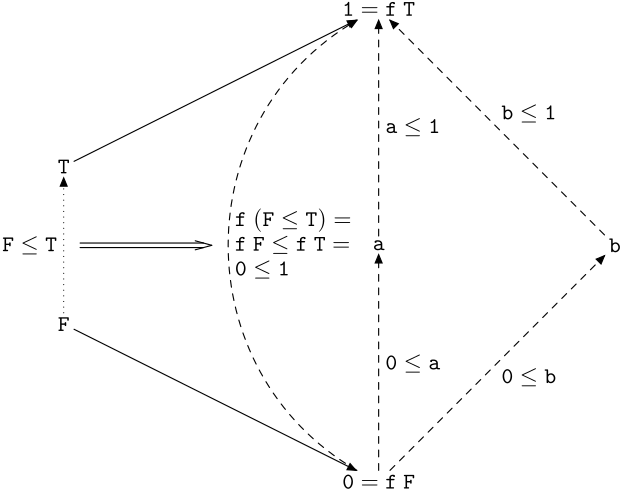
\includegraphics[scale=0.33]{../images/cat-bool-m2.png}
\end{center}
\caption{Graph of |f :: Bool -> M2|}
\label{fig:f-bool-to-m2}
\end{figure}

The graph of |f| is on \cref{fig:f-bool-to-m2}. Dotted and dashed lines are arrows
in |Bool| and |M2| respectively.
We can see on figure, that |f| indeed gives a picture of |Bool| in |M2|.

In \Haskell\ we have only written
a mapping of objects, |True| and |False|. The mapping of arrows is something
we need to check, to be able to claim that |f| is a functor, and therefore
a monotone function. The other way around, there are mappings from 
|Bool| to |M2| which aren't monotone, and aren't functors.

In this section we went backwards. More principal approach would been to first
consider functors between poset categories. The monotonicity requirement is
implied by first functor requirement. This is a power of category
theory. When you look for something, category theory tells you which
properties it should have. Once you find something which satisfies
the requirements, you know that it's the right one (up to an isomorphism).

\rule{\textwidth}{1pt}
\ldots
\rule{\textwidth}{1pt}

Exponential lattices with |M2| are pretty. |ZHO -> M2| (\cref{fig:zho2m2})
has nice planar graph. \ldtos . Yet the final stress test is
|(ZHO -> ZHO) -> ZHO|, or $\mathtt{ZHO}^{\mathtt{ZHO}^\mathtt{ZHO}}$ is on \cref{fig:big}.
A beautiful monster.

\begin{figure}[ht]
\begin{center}
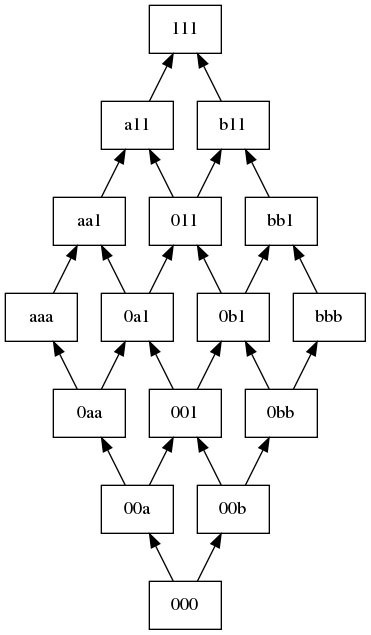
\includegraphics[scale=0.3]{../images/lattice-zho2m2.png}
\end{center}
\caption{|ZHO -> M2| lattice}
\label{fig:zho2m2}
\end{figure}

\begin{figure}[ht]
\begin{center}
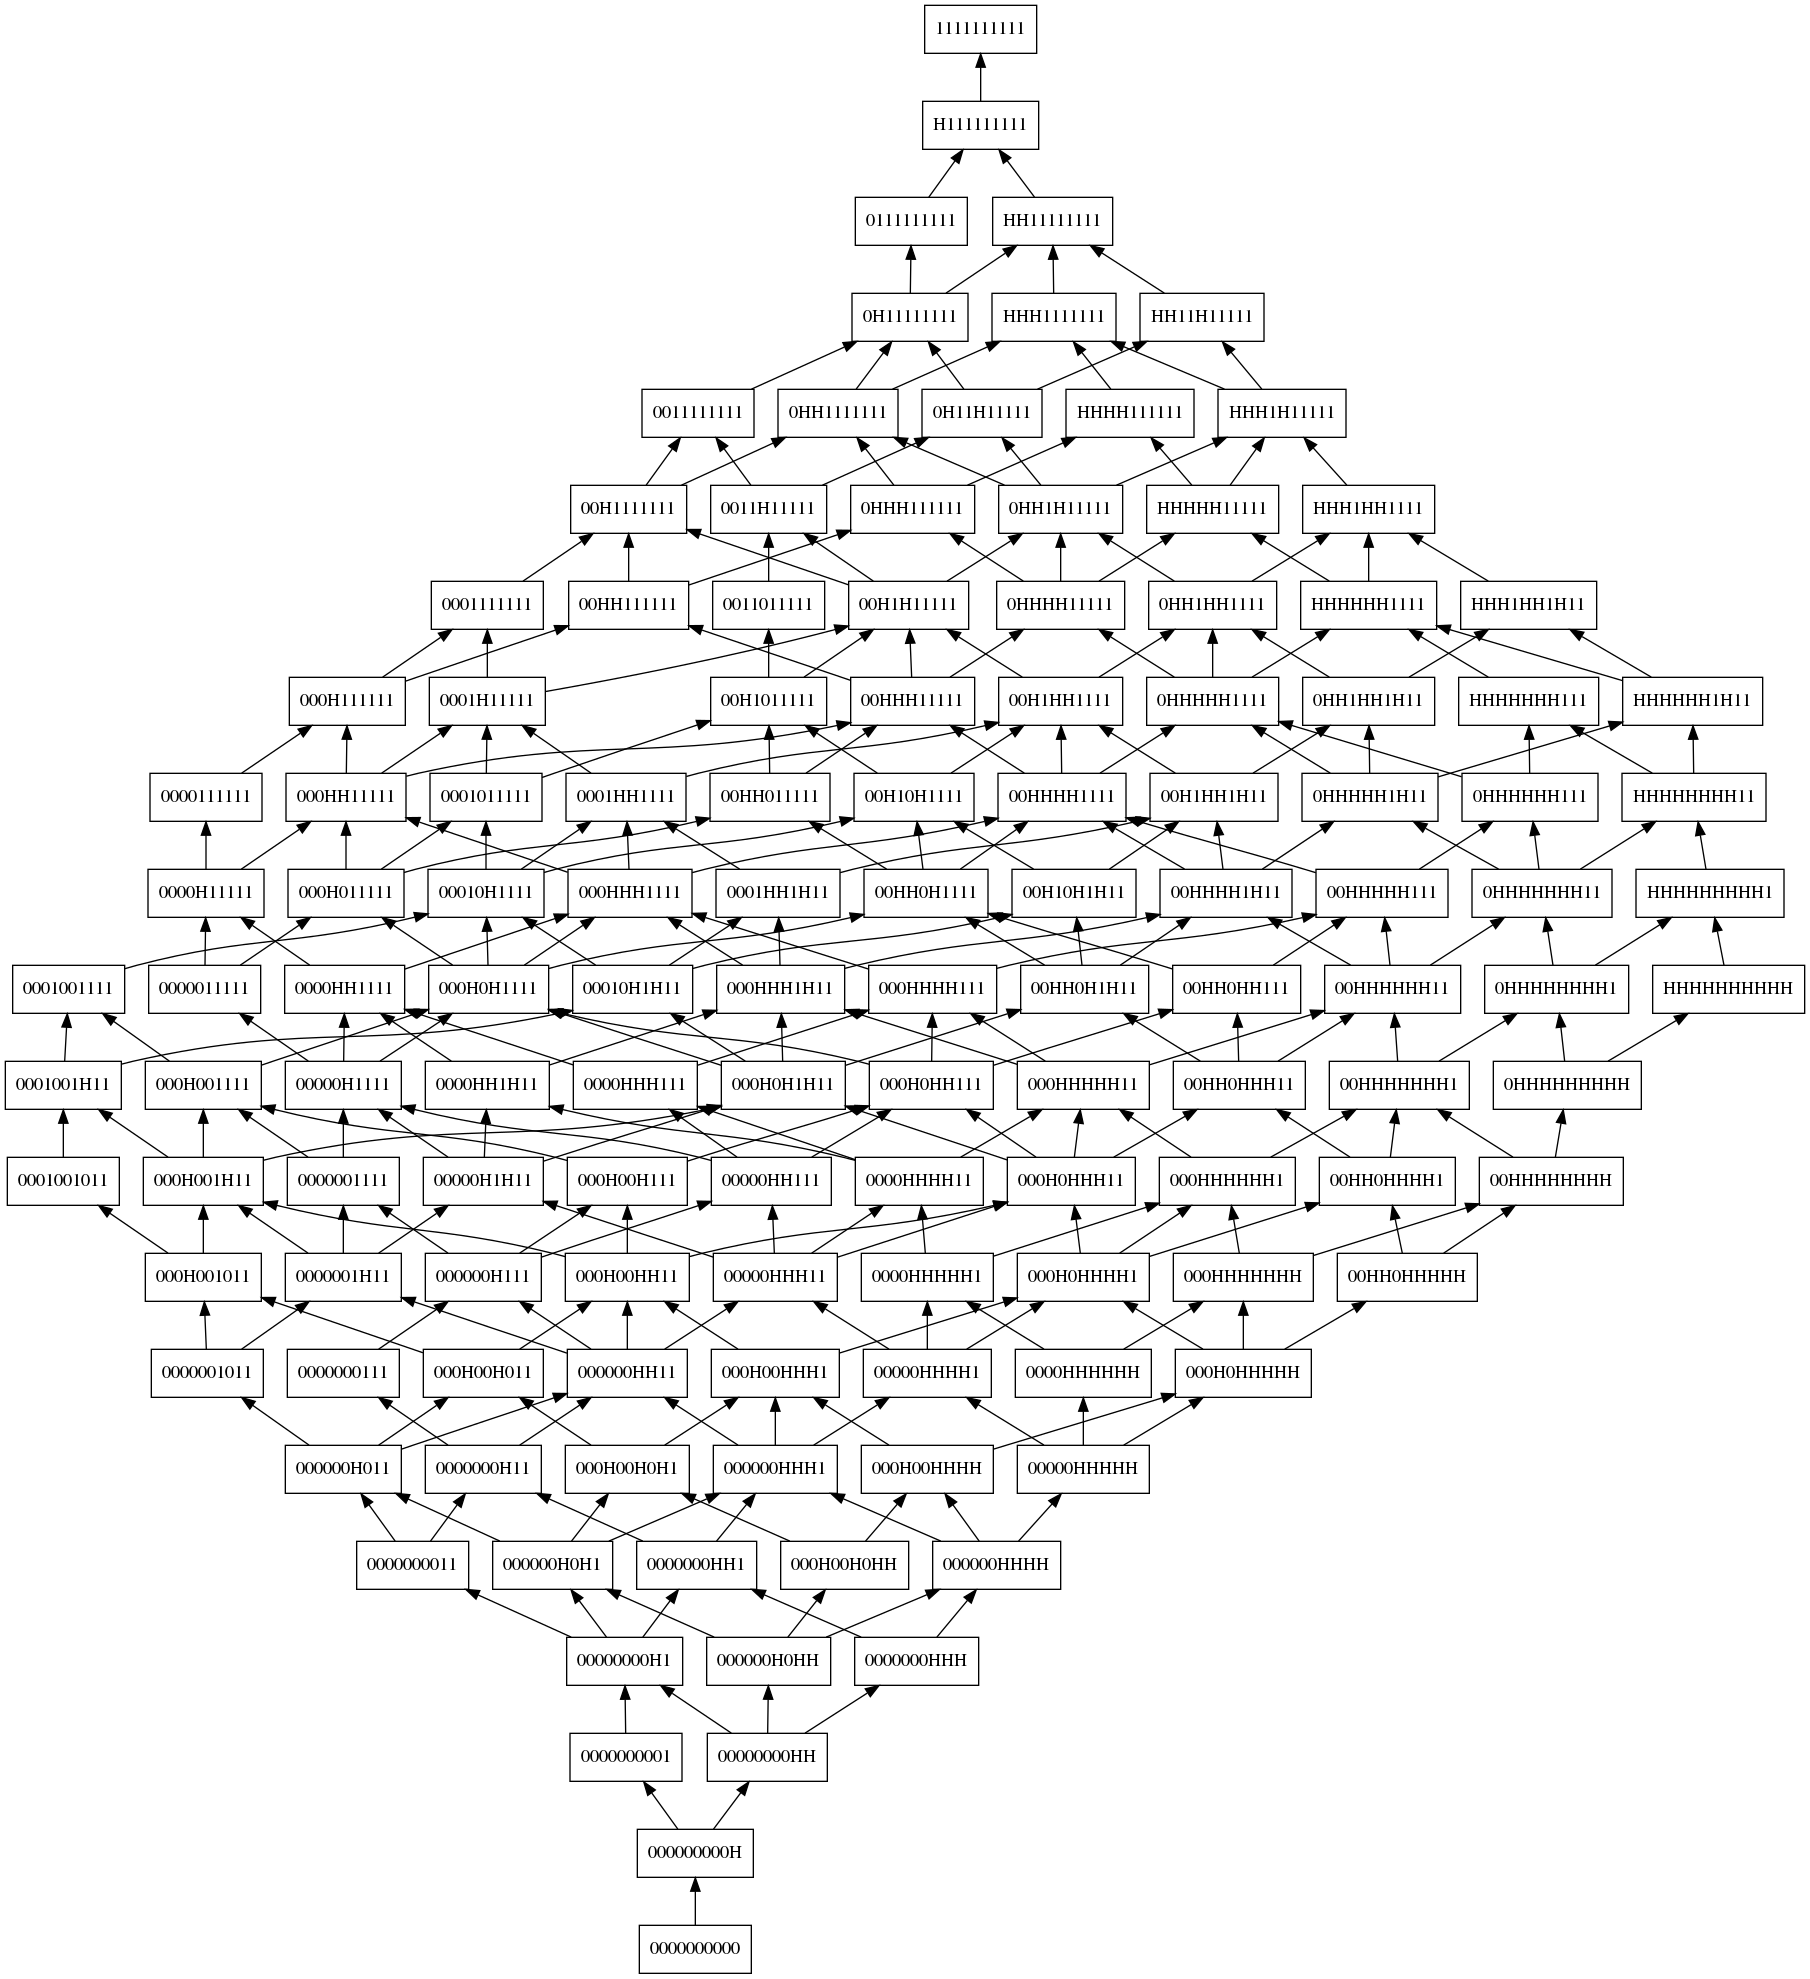
\includegraphics[scale=0.15]{../images/lattice-big.png}
\end{center}
\caption{|(ZHO -> ZHO) -> ZHO| lattice}
\label{fig:big}
\end{figure}

\end{document}
